\subsection*{Character importance}

The characters used in the cluster analysis have each different importance in distinguish between signature types.
Those characters which spatial distribution most closely matches the distribution of signatures
can be seen as more important that those that are seemingly random or mostly invariant (as some of the land cover classes are).
Unpacking the importance of individual characters from K-Means clustering cannot be done directly, but
a useful method is to train a supervised model, in our case Random Forest, designed to predict individual
signature types from input data. Such a model then provides a feature importance - a relative measure of
a strenght of each character in distinguishing between the types. The results of this approach are shown in
a table \ref{tab:imp}. As you can see, form-based characters dominate the top 10 characters but it is worth
noting that these top 10 characters together bear only 0.196 of the overall importance.

\begin{table}
\begin{tabular}{lr}
    \toprule
    {} &  relative importance \\
    \midrule
    covered area ratio of ETC (Q1)             &             0.036944 \\
    covered area ratio of ETC (Q2)             &             0.031717 \\
    perimeter-weighted neighbours of ETC (Q2)  &             0.023476 \\
    mean inter-building distance (Q2)          &             0.016662 \\
    area of ETC (Q3)                           &             0.016005 \\
    area covered by node-attached ETCs (Q3)    &             0.014813 \\
    longest axis length of ETC (Q2)            &             0.014501 \\
    weighted reached enclosures of ETC (Q1)    &             0.014115 \\
    reached area by neighbouring segments (Q3) &             0.014000 \\
    reached area by neighbouring segments (Q1) &             0.013904 \\
    \bottomrule
\end{tabular}
\caption{\label{tab:imp}Relative importance of top 10 most important characters in
predicting spatial signature types using the Random Forest model.}
\end{table}

A similar exercise can be done on a level of individual clusters, with a binary Random Forest model trained
to distingish that particular class from the other. Resulting relative importance of top 10 characters for each signature type
is presented in a table \ref{tab:imp_cls}. While it is clear that form-based characters still dominate the prediction,
the more urban signature types are, the higher the importance of function seems to be. Complete tables
with all characters are availble as online tables 1 and 2.

\begin{table}
    \begin{tabular}{lrlrlrlrlrlrlrlrlrlrlrlrlrlrlrlr}
        \toprule
                                         Wild countryside & \multicolumn{2}{l}{Countryside agriculture} & \multicolumn{2}{l}{Gridded residential quarters} & \multicolumn{2}{l}{Accessible suburbia} & \multicolumn{2}{l}{Connected residential neighbourhoods} & \multicolumn{2}{l}{Urban buffer} & \multicolumn{2}{l}{Open sprawl} & \multicolumn{2}{l}{Warehouse/Park land} & \multicolumn{2}{l}{Local urbanity} & \multicolumn{2}{l}{Dense residential neighbourhoods} & \multicolumn{2}{l}{Disconnected suburbia} & \multicolumn{2}{l}{Dense urban neighbourhoods} & \multicolumn{2}{l}{Regional urbanity} & \multicolumn{2}{l}{Metropolitan urbanity} & \multicolumn{2}{l}{Concentrated urbanity} & \multicolumn{2}{l}{Hyper concentrated urbanity} \\
                                                     name & rel. importance &                                               name & rel. importance &                                               name & rel. importance &                                         name & rel. importance &                                               name & rel. importance &                                               name & rel. importance &                                        name & rel. importance &                                               name & rel. importance &                                               name & rel. importance &                                             name & rel. importance &                                               name & rel. importance &                                               name & rel. importance &                                               name & rel. importance &                                               name & rel. importance &                                               name & rel. importance &                                               name & rel. importance \\
        \midrule
                          longest axis length of ETC (Q1) &        0.196609 &                     covered area ratio of ETC (Q1) &        0.154212 &             local closeness of street network (Q3) &        0.095416 &      weighted reached enclosures of ETC (Q3) &        0.063690 &                    cell alignment of building (Q1) &        0.028481 &            area covered by neighbouring cells (Q2) &        0.071780 &   reached area by local street network (Q1) &        0.058349 &                        elongation of building (Q1) &        0.033986 &                         perimeter of building (Q2) &        0.101218 & centroid - corner mean distance of building (Q2) &        0.036962 & local proportion of cul-de-sacs of street netwo... &        0.023643 &                         perimeter of building (Q2) &        0.106663 & centroid - corner distance deviation of buildin... &        0.115378 &      equivalent rectangular index of building (Q2) &        0.110605 &                              area of building (Q1) &        0.128233 &                     covered area ratio of ETC (Q2) &        0.154124 \\
                           covered area ratio of ETC (Q2) &        0.151118 &                     covered area ratio of ETC (Q2) &        0.144279 &             local closeness of street network (Q2) &        0.046007 & reached ETCs by tessellation contiguity (Q3) &        0.062061 & local proportion of 4-way intersections of stre... &        0.022801 &                     covered area ratio of ETC (Q2) &        0.049986 &  reached area by neighbouring segments (Q1) &        0.033786 &   centroid - corner mean distance of building (Q3) &        0.028038 &      equivalent rectangular index of building (Q1) &        0.093518 & centroid - corner mean distance of building (Q3) &        0.030172 &            local meshedness of street network (Q3) &        0.021436 &   centroid - corner mean distance of building (Q2) &        0.084484 &   centroid - corner mean distance of building (Q2) &        0.088275 &   centroid - corner mean distance of building (Q2) &        0.087236 & Workplace population [Distribution, hotels and ... &        0.099872 &          Workplace population [Manufacturing] (Q2) &        0.143669 \\
                           covered area ratio of ETC (Q1) &        0.145754 &                  mean inter-building distance (Q2) &        0.078928 &                        perimeter of enclosure (Q1) &        0.044369 & reached area by tessellation contiguity (Q2) &        0.047628 &                    cell alignment of building (Q2) &        0.017361 & mean distance to neighbouring nodes of street n... &        0.048812 &     area covered by node-attached ETCs (Q2) &        0.023548 &                        elongation of building (Q2) &        0.025310 &   centroid - corner mean distance of building (Q2) &        0.082040 &                            area of building (Q3) &        0.029425 &            local meshedness of street network (Q2) &        0.020520 &                         perimeter of building (Q3) &        0.082203 &                        squareness of building (Q3) &        0.082130 & centroid - corner distance deviation of buildin... &        0.080684 & Workplace population [Financial, real estate, p... &        0.076751 &                  Workplace population [Other] (Q2) &        0.101678 \\
                                         area of ETC (Q2) &        0.096485 &                                   area of ETC (Q2) &        0.072977 &                             area of enclosure (Q2) &        0.037296 &                             area of ETC (Q2) &        0.045100 &                             area of enclosure (Q2) &        0.017232 &                     covered area ratio of ETC (Q1) &        0.046002 &              covered area ratio of ETC (Q2) &        0.022004 &              circular compactness of building (Q1) &        0.019596 &                        squareness of building (Q3) &        0.054375 &                                  Population (Q3) &        0.028051 &      equivalent rectangular index of building (Q1) &        0.020273 &                              area of building (Q2) &        0.066331 & Workplace population [Financial, real estate, p... &        0.071195 &                           corners of building (Q2) &        0.071910 &                  Workplace population [Other] (Q2) &        0.075844 & Workplace population [Distribution, hotels and ... &        0.081796 \\
                perimeter-weighted neighbours of ETC (Q3) &        0.075078 &            area covered by node-attached ETCs (Q2) &        0.066916 &             local closeness of street network (Q1) &        0.036698 &   reached ETCs by neighbouring segments (Q1) &        0.036865 &                            orientation of ETC (Q2) &        0.016519 &         reached area by neighbouring segments (Q1) &        0.038292 &   local node density of street network (Q3) &        0.018821 & centroid - corner distance deviation of buildin... &        0.017568 &                              area of building (Q2) &        0.051383 &                       perimeter of building (Q2) &        0.025995 &              circular compactness of building (Q1) &        0.019361 &                                    Population (Q3) &        0.039538 &                         perimeter of building (Q2) &        0.065223 & Workplace population [Financial, real estate, p... &        0.060205 & Workplace population [Distribution, hotels and ... &        0.070516 &                     covered area ratio of ETC (Q1) &        0.079165 \\
               reached area by neighbouring segments (Q1) &        0.048869 & mean distance to neighbouring nodes of street n... &        0.066150 &            weighted reached enclosures of ETC (Q3) &        0.031708 &   reached ETCs by neighbouring segments (Q2) &        0.029904 &      equivalent rectangular index of building (Q1) &        0.016281 &                   circular compactness of ETC (Q2) &        0.034693 &  reached area by neighbouring segments (Q2) &        0.018065 &                         perimeter of building (Q3) &        0.017147 & centroid - corner distance deviation of buildin... &        0.044975 &                            area of building (Q2) &        0.022935 &                                    Population (Q1) &        0.017855 &                        squareness of building (Q3) &        0.039269 &                         perimeter of building (Q3) &        0.057863 & Workplace population [Distribution, hotels and ... &        0.051041 & Workplace population [Financial, real estate, p... &        0.060396 &          Workplace population [Manufacturing] (Q3) &        0.074537 \\
             reached area by tessellation contiguity (Q1) &        0.018289 &         reached area by neighbouring segments (Q1) &        0.062776 & local proportion of 4-way intersections of stre... &        0.020617 &    reached ETCs by local street network (Q2) &        0.026220 & local proportion of 4-way intersections of stre... &        0.014317 &            area covered by neighbouring cells (Q1) &        0.033082 &              covered area ratio of ETC (Q1) &        0.018036 &                       width of street profile (Q2) &        0.016790 & Workplace population [Financial, real estate, p... &        0.044019 &                      perimeter of enclosure (Q1) &        0.020672 &                        elongation of building (Q2) &        0.016115 & centroid - corner distance deviation of buildin... &        0.034407 &                              area of building (Q2) &        0.050349 &                         perimeter of building (Q2) &        0.046511 &          Workplace population [Manufacturing] (Q2) &        0.054662 &   centroid - corner mean distance of building (Q2) &        0.070363 \\
                                         area of ETC (Q3) &        0.015991 &       Land cover [Discontinuous urban fabric] (Q2) &        0.055444 &            area covered by node-attached ETCs (Q1) &        0.019211 &    perimeter-weighted neighbours of ETC (Q1) &        0.023718 &                        perimeter of enclosure (Q1) &        0.014305 &         buildings per meter of street segment (Q2) &        0.032175 &                      area of enclosure (Q2) &        0.017156 &              circular compactness of building (Q2) &        0.016306 & Workplace population [Distribution, hotels and ... &        0.035144 &                    orientation of enclosure (Q2) &        0.017636 &         reached area by neighbouring segments (Q2) &        0.015907 & Workplace population [Financial, real estate, p... &        0.029293 & Workplace population [Distribution, hotels and ... &        0.048963 &                        squareness of building (Q3) &        0.039035 &                         perimeter of building (Q2) &        0.046941 &                         perimeter of building (Q2) &        0.054542 \\
        mean distance between neighbouring buildings (Q2) &        0.015013 &          perimeter-weighted neighbours of ETC (Q2) &        0.021903 &            area covered by node-attached ETCs (Q2) &        0.018326 & reached area by tessellation contiguity (Q1) &        0.022821 & local proportion of cul-de-sacs of street netwo... &        0.013748 &       reached area by tessellation contiguity (Q1) &        0.029531 & compactness-weighted axis of enclosure (Q3) &        0.016709 &       reached area by tessellation contiguity (Q1) &        0.016248 &                         perimeter of building (Q3) &        0.033695 &                       perimeter of building (Q3) &        0.016561 &            area covered by edge-attached ETCs (Q3) &        0.015526 &      equivalent rectangular index of building (Q1) &        0.017548 &                           corners of building (Q3) &        0.029268 & Workplace population [Financial, real estate, p... &        0.029708 &   centroid - corner mean distance of building (Q2) &        0.044694 &                    openness of street profile (Q2) &        0.031258 \\
                        mean inter-building distance (Q2) &        0.010559 &                    longest axis length of ETC (Q2) &        0.020504 &            weighted reached enclosures of ETC (Q2) &        0.016607 &    reached ETCs by local street network (Q1) &        0.020275 &                      orientation of enclosure (Q1) &        0.013305 &            area covered by node-attached ETCs (Q3) &        0.027952 &                            area of ETC (Q2) &        0.015707 &                         perimeter of building (Q2) &        0.014735 &                              area of building (Q1) &        0.022769 &                           area of enclosure (Q1) &        0.015454 &              circular compactness of building (Q2) &        0.015257 &                  Workplace population [Other] (Q2) &        0.016284 & centroid - corner distance deviation of buildin... &        0.020625 &   centroid - corner mean distance of building (Q1) &        0.018957 &        Land cover [Non-irrigated arable land] (Q1) &        0.025912 &                                          NDVI (Q3) &        0.027406 \\
        \bottomrule
        \end{tabular}
        \caption{\label{tab:imp_cls}Relative importance of top 10 most important characters for each signature type in
        predicting using the Random Forest model.}
\end{table}

\subsection*{Comparison}

Spatial signatures are unique as a classification method, limiting the potential
validation. Therefore, we rahter present a comparison of signatures and ancillary datasets capturing
conceptually similar aspects of the environment. We compare the signatures with four of
such datasets, each focusing on a different classification perspective, but all related
to our classification to a degree when we can assume there will be a measurable level of
association between the two:

\begin{itemize}
    \item WorldPop settlement patterns of building footprints (2021)\cite{jochem2021tools}
    \item Classification of Multidimensional Open Data of Urban Morphology (MODUM) (2015)\cite{alexiou2016}
    \item Copernicus Urban Atlas (2018)\cite{eea2018}
    \item Local Climate Zones (2019)\cite{demuzere2019mapping}
\end{itemize}


\subsection*{Comparison approach}
% General method of validation
    % data transfer (one or the other way depending on feasibility) chi-squared
    % statistic Cramer's V
All datasets, spatial signatures and those selected for a comparison contain a
categorical classification of space linked to their unique geometry. The first
requirement to be able to compare data products is to transfer their
information to the same geometry. We take two approaches for this step,
depending on the dataset we are comparing the signatures with:
an interpolation of one set of polygon-based data to another (input to ETCs);
or the conversion of
spatial signatures to the raster representation matching an input raster,
which is computationally more efficient when one of the layers is already a raster. The second
step is a statistical comparison of two sets of classification labels, one representing
spatial signature typology and the other comparison classes. We use contingency tables
and Pearson's $\chi^{2}$ test to determine whether the frequencies of observed
(signature types) and expected (comparison types) labels significantly differ in one or
more categories. Furthermore, we use Cramér's $V$ statistics\cite{cramer2016mathematical} to assess the strength of
the association.

\subsection*{WorldPop settlement patterns of building footprints}
% - WorldPop (Spsig)
    % description of dataset + figure
WorldPop settlement patterns of building footprints dataset aims to derive a typology of
morphological patterns based on a gridded approach with cells of
100x100m, and building footprints. Authors measure six morphometric characters
linked to the grid cells and use them as input for an unsupervised clustering
algorithm leading to a six-class typology.
    % expectations regarding similarity
As the classification is dependent on building footprints, grid cells that do
not contain any information on the building-based pattern are treated as missing in the
final data product. For the comparison, this \textit{missing}
category is treated as a single class. It is assumed that the top-level large scale
patterns detected by the WorldPop method and spatial signatures will provide similar
results. However, there will be differences caused by the inclusion of function in spatial
signatures, higher granularity of both initial spatial units and the resulting
classification (6 vs 19 classes).

Signature typology is rasterized and linked to the WorldPop grid. The resulting
contingency table is shown in Figure \ref{fig:crosstab_worldpop}. There is a significant relationship between
two typologies, $\chi^{2} (114, N = 22993921) = 13341832, p < .001$. The strength of
association measured as Cram\'{e}r's $V$ is $0.311$, indicating moderate association.
The contingency table shows that WorldPop classes tend to be linked to groups of
signature types of a similarly degree of urbanity. A WorldPop class 15 is "undefined" due
to the lack of building footprints in the area, therefore overlapping a large portion of
signatures.
    % results + contingency table figure
The difference between classifications is likely driven by two main aspects - one is the different
number of classes. We can see that WorldPop classes tend to cluster wihtin a limited number of
signature types and vice versa. The only exception is allocation of signature types into classes 4 and 6,
which seems to heavily overlap. That is possibly caused by the second aspect - inclusion of function. Both
classes 4 and 6 tend to be outside of city centres but still within urban areas. While it is
the footprint-based form that is driving the difference between them, signatures in the same
area are often disntiguished by function and varies access to amenities and services.

\begin{figure}
    \centering
    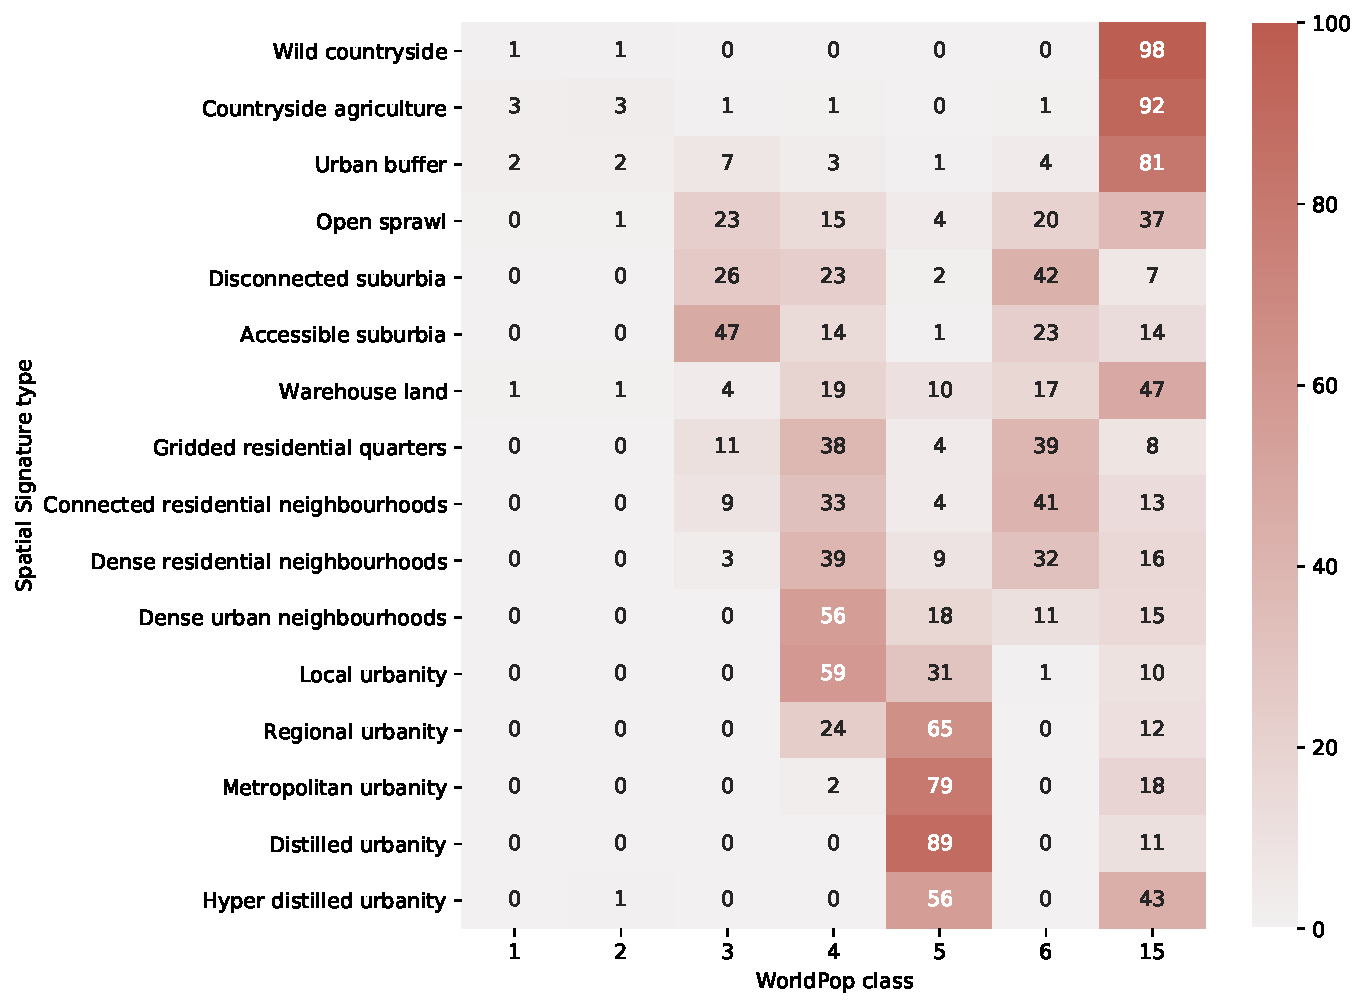
\includegraphics[width=.8\linewidth]{fig/crosstab_worldpop.pdf}
    \caption{Contingency table showing frequencies (in \%) of WorldPop classes within signature types.}
    \label{fig:crosstab_worldpop}
\end{figure}

\subsection*{MODUM}
% - MODUM (Spsig)
    % description of dataset + figure
Multidimensional Open Data Urban Morphology (MODUM) classification describes a typology
of neighbourhoods derived from 18 indicators capturing built environment as streets,
railways or parks, linked to the Census Output Area geometry. The classification
identifies 8 types of neighbourhoods.
    % expectations regarding similarity
Compared to the WorldPop classification, MODUM takes into account more features of
the built environment than building footprints, which makes it conceptually closer to the
spatial signatures. However, it is still focusing predominantly on the form component,
although there are some indicators that would be classified as function within the
signatures framework (e.g. population). The MODUM method uses a different way of
capturing context compared to the signatures, which leads to some classes being
determined predominantly by a single character. For example, the \textit{Railway Buzz} type
forms a narrow strip around the railway network, which is an effect signatures avoid.
    % results + contingency table figure
MODUM typology is available only for England and Wales. Therefore the comparison takes
into account only ETCs covering the same area. The classification is linked to the
ETC geometry is based on the proportion (the type covering the largest portion of ETC is
assigned). The resulting contingency table is shown in Figure \ref{fig:crosstab_modum}. There is a
significant relationship between two typologies, $\chi^{2} (152, N = 13067584) =
13938867, p < .001$. The strength of association measured as Cramér's $V$ is $0.300$,
indicating moderate association of very similar levels we have seen above. The
contingency table indicates similar relationships, where a single MODUM class overlaps a
group of signature types. However, the groups tend to be well defined and formed based
on the similarity of types. Signature types are minimally present in MODUM classes driven
by a single character (\textit{Railway Buzz}, \textit{Waterside Settings},
\textit{High Street and Promenades}), suggesting the more balanced weight of characters.


\begin{figure}
    \centering
    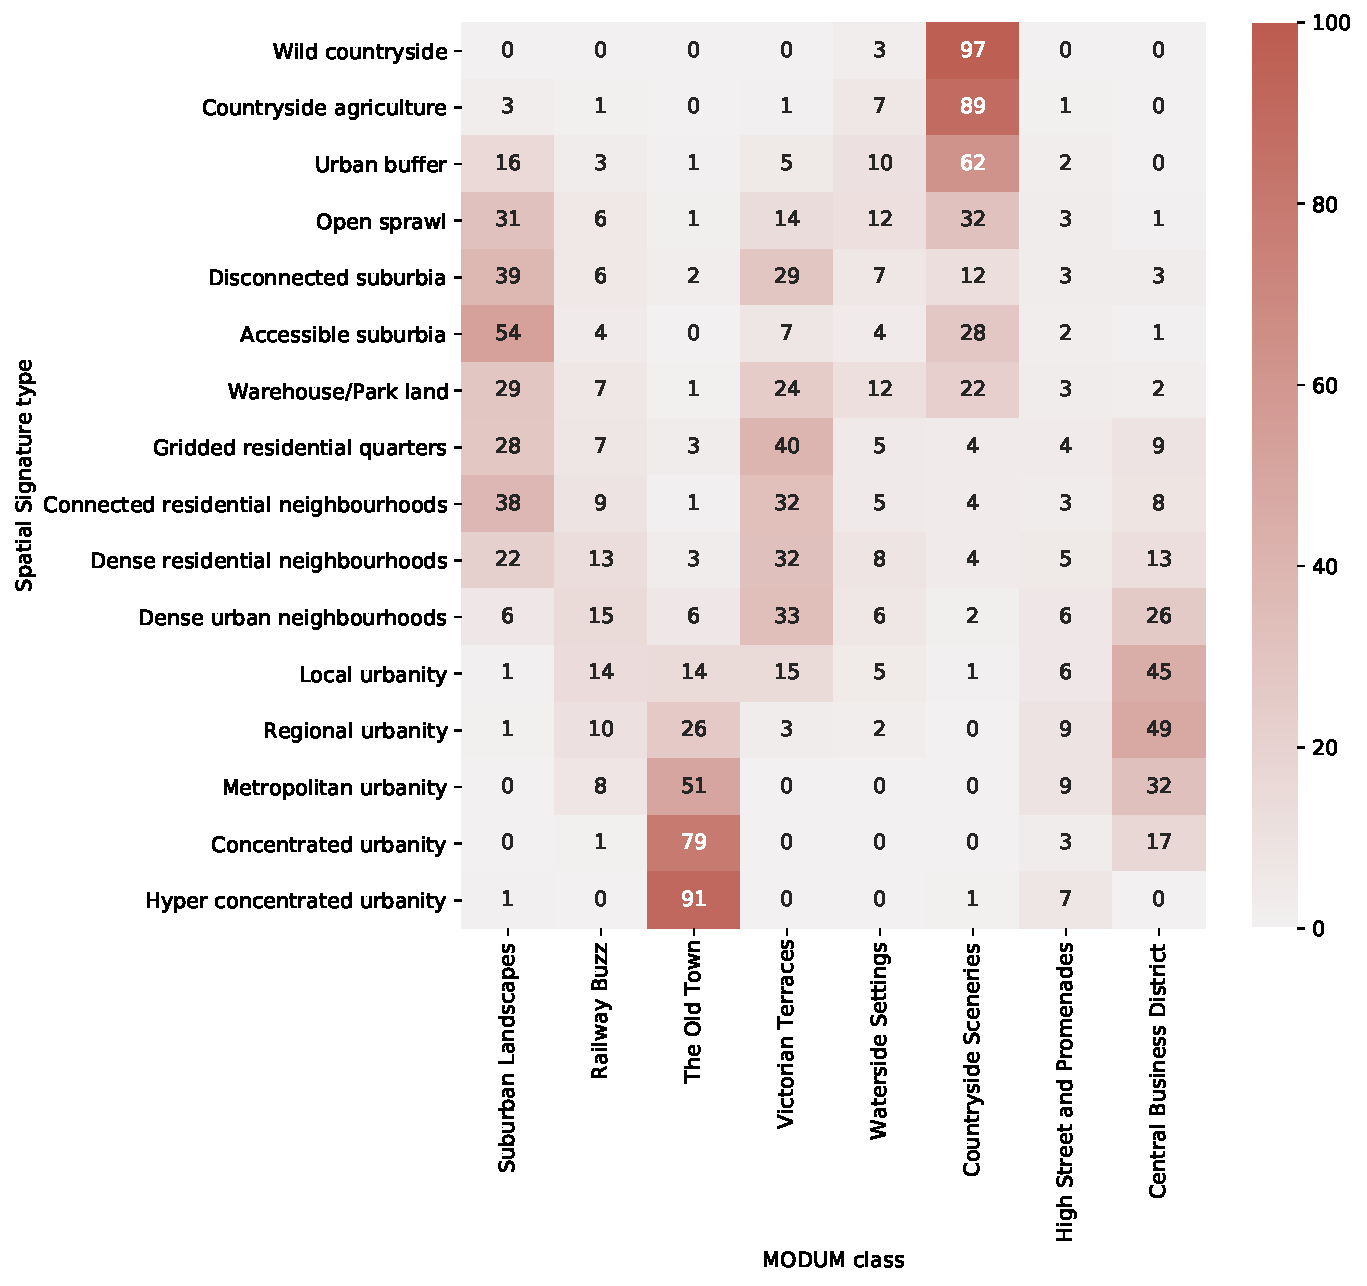
\includegraphics[width=.8\linewidth]{fig/crosstab_modum.pdf}
    \caption{Contingency table showing frequencies (in \%) of MODUM classes within signature types.}
    \label{fig:crosstab_modum}
\end{figure}

\subsection*{Copernicus Urban Atlas}
% - Urban atlas (Spsig)
    % description of dataset + figure
Copernicus Urban Atlas is the least similar of the comparison datasets. It is a
high-resolution land use classification of functional urban areas derived primarily from
Earth Observation data enriched by other reference data as OpenStreetMap or topographic
maps. Its smallest spatial unit in urban areas is 0.25 ha and 1 ha in rural areas,
defined primarily by physical barriers. It identifies
27 predefined classes using the supervised method.
    % expectations regarding similarity
The majority of urban areas is classified as urban fabric further distinguished based on
continuity and density resulting in six classes of the urban fabric. The classification does
not consider the type of the pattern or any other aspect. Furthermore, it does not take
into account what signatures call \textit{context} as each spatial unit is
classified independently, which in some cases leads to the high heterogeneity of
classification within a small portion of land. Signatures take a different approach.
Consequently, it is expected that the similarity between the two will be limited.
    % results + contingency table figure
Urban Atlas is available only for functional urban areas (FUA), leaving rural areas
unclassified. Comparison then applies to FUAs only. The classification is linked to the
ETC geometry based on the proportion (the type covering the largest portion of ETC is
assigned). The resulting contingency table is shown in Figure \ref{fig:crosstab_ua}. There is a
significant relationship between two typologies, $\chi^{2} (450, N = 8396642) = 5229900,
p < .001$. The strength of association measured as Cramér's $V$ is $0.186$, indicating
a weak association. The contingency table shows the difference in the aim of spatial
signatures and that of Urban Atlas with a majority of signatures being linked to a few
of Urban Atlas classes. Within relevant classes, we see a tendency of signature types to
cluster within Urban Atlas classes based on the level of urbanity, albeit not as strong
as in the previous two cases.
The main reason behind such a large difference are the aims of both classifications. While
the Copernicus Urban Atlas attemps to capture land cover, resulting in a large number
of non-urban classes, spatial signatures are aimed at urban environment with 13 out of 16
classes covering primarily urbanised areas.

\begin{figure}
    \centering
    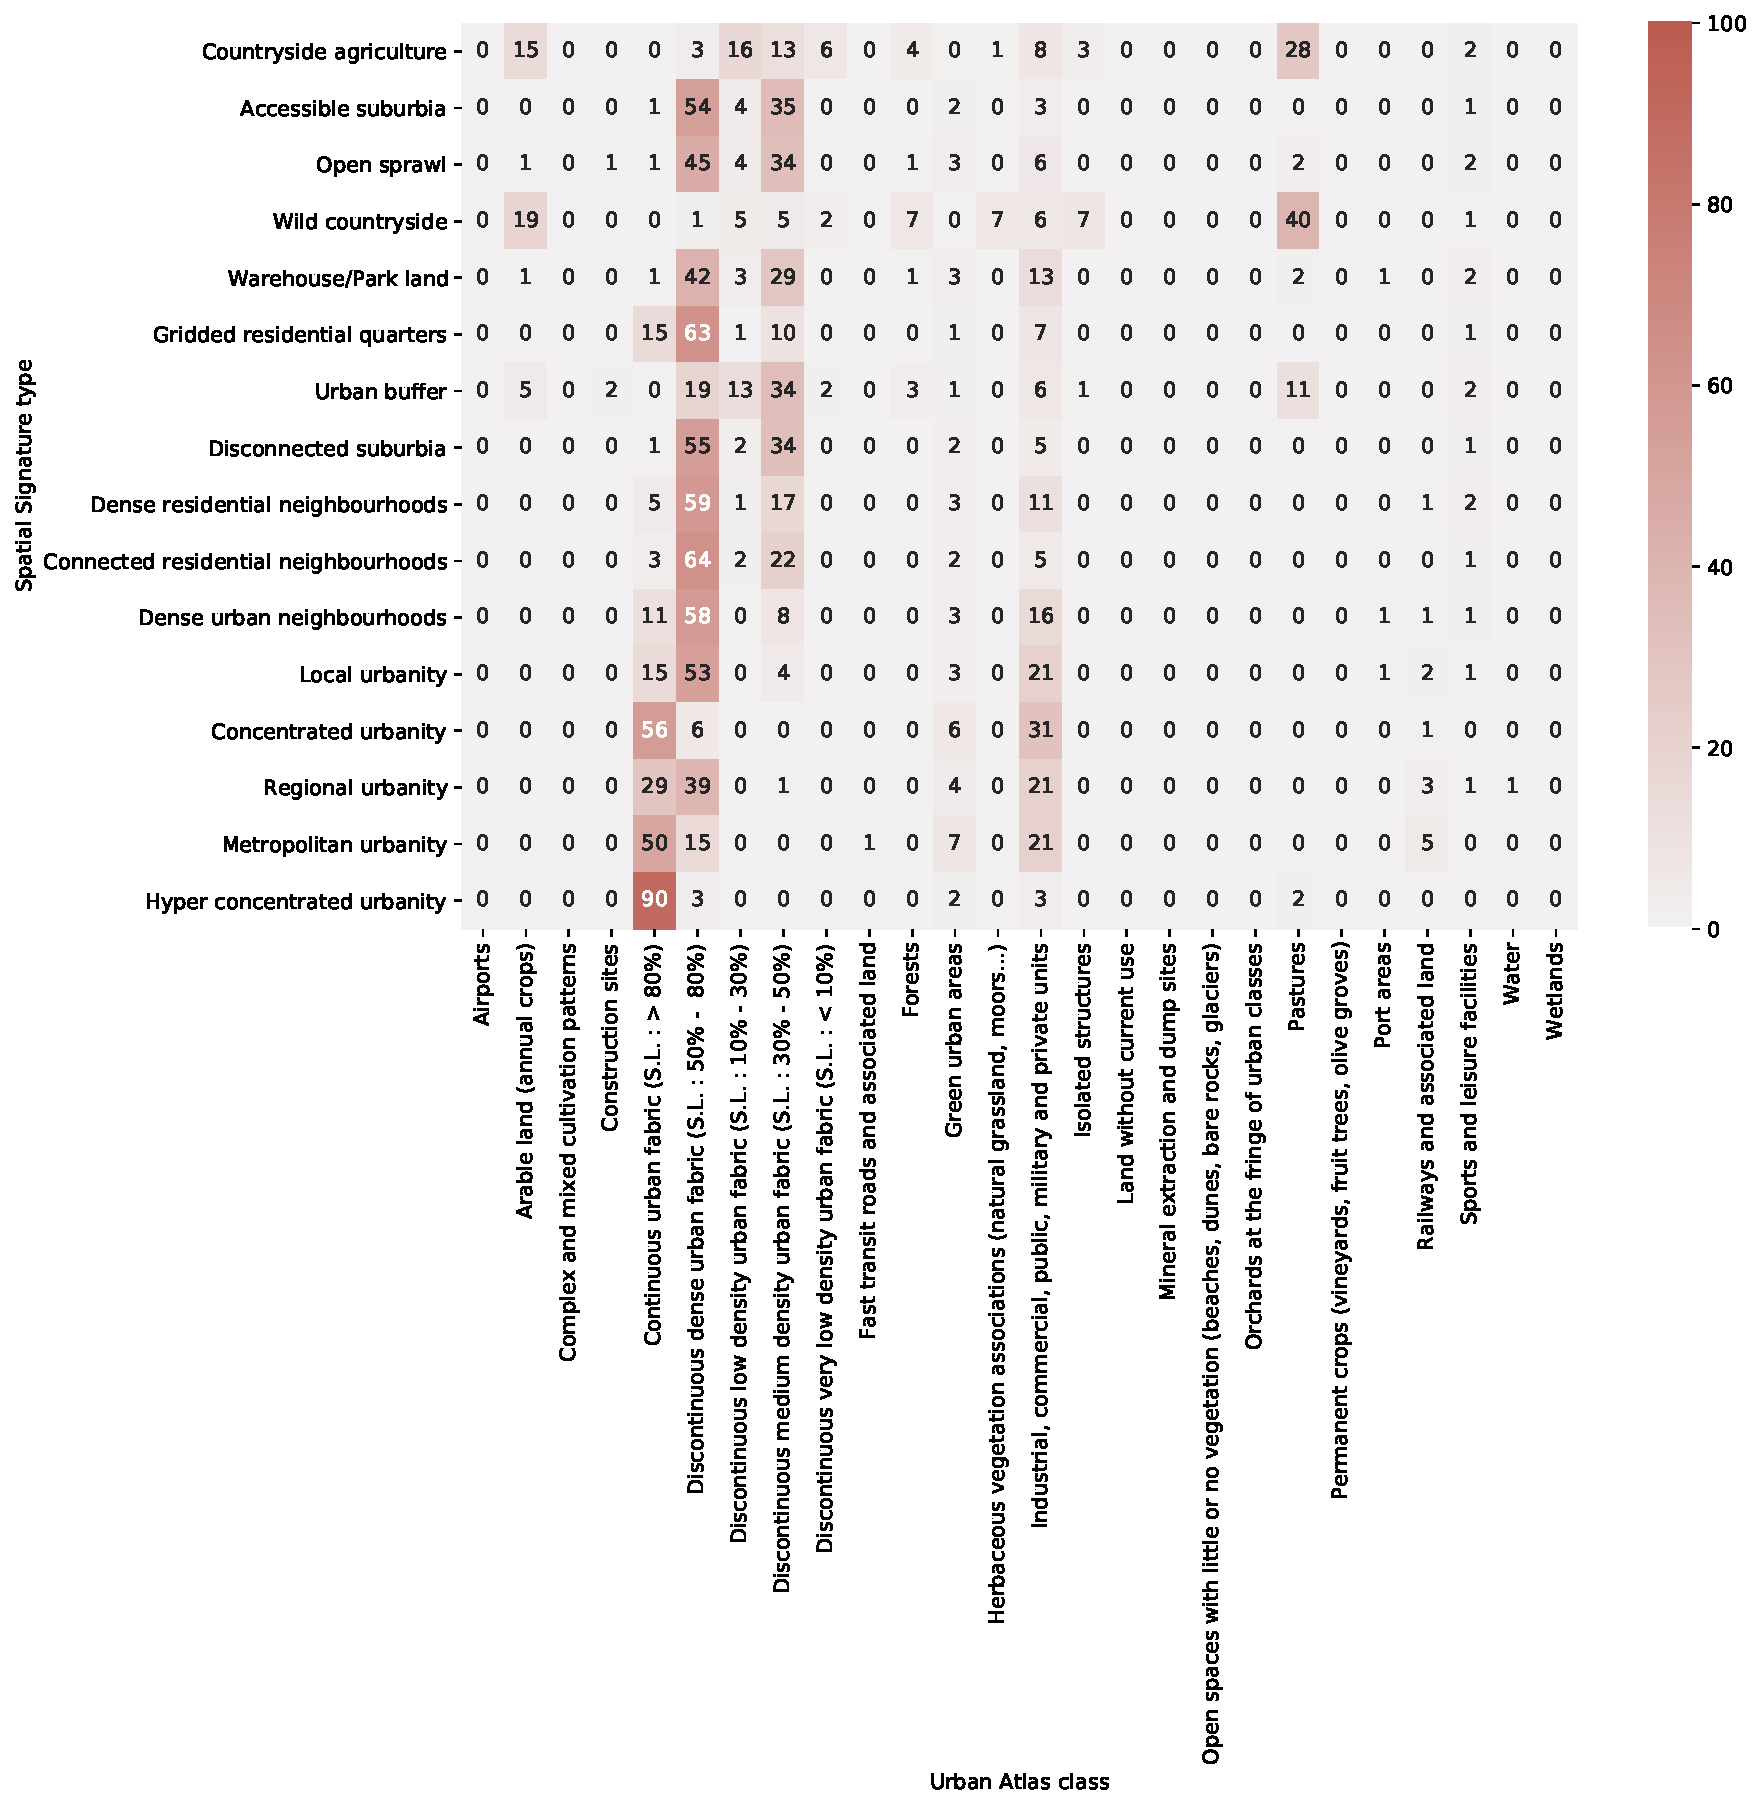
\includegraphics[width=\linewidth]{fig/crosstab_ua.pdf}
    \caption{Contingency table showing frequencies (in \%) of Urban Atlas classes within signature types.}
    \label{fig:crosstab_ua}
\end{figure}

\subsection*{Local Climate Zones}
% - Local climate zones (Spsig)
    % description of dataset + figure
Local climate zones (LCZ) are conceptual classes originally designed to support study of urban
climate as temperature. It consists of 17 classes of which 10 can be classified as urban
and 7 and natural ones. In the context of Great Britain, the dataset used in this study
does not contain 2 of them, \textit{Lightweight low-rise} and \textit{Compact highrise}
as they are not present in the British landscape. The datasets produced by
\cite{demuzere2019mapping} released LCZs in a 100 meters grid based on the 2016 data. As
the LCZs are remotely sensed in this case, authors report overall average accuracy of 80 \%.
    % expectations regarding similarity
As a conceptual classification aimed to cover all possible types of primariliy urban climate zones globally,
LZCs may not be optimal when looking into a single country with specific history of urban
development. This is furhter indicated by classes that are missing. It is therefore likely
that large parts of British cities will fall into only a few of LCZ classes, while being representated
by a much larger number of signature types.
    % results + contingency table figure

Signature typology is rasterized and linked to the LCZ grid.
The resulting contingency table is shown in Figure \ref{fig:crosstab_lcz}. There is a
significant relationship between two typologies, $\chi^{2} (225, N = 16203338) = 18467242,
p < .001$. The strength of association measured as Cramér's $V$ is $0.276$, indicating
a modest to weak association, close to values we've seen in first two cases. As expected,
urban signature types are clustered primarily within \textit{Compact midrise} and
\textit{Open lowrise} LCZs, while non-urban signatures mostly fall into the \textit{Low plants} LCZ.

The difference between signatures and LCZs can be accounted to two aspects. One, as we've seen
before is the inclusion of function in spatial signatures, differentiating e.g. LCZ's \textit{Open lowrise} into
many signature types. The other is data-driven nature of signatures compared to conceptual LCZs,
where differences in signature types are below the resolution capability of simple matrix composed of
density and compactness levels. On the other, it is encouraging to see that most of signature types
fall predominantly in a single LCZ class, suggesting that while both classifications are built differently,
they are able to capture similar large-scale patterns in cities.

\begin{figure}
    \centering
    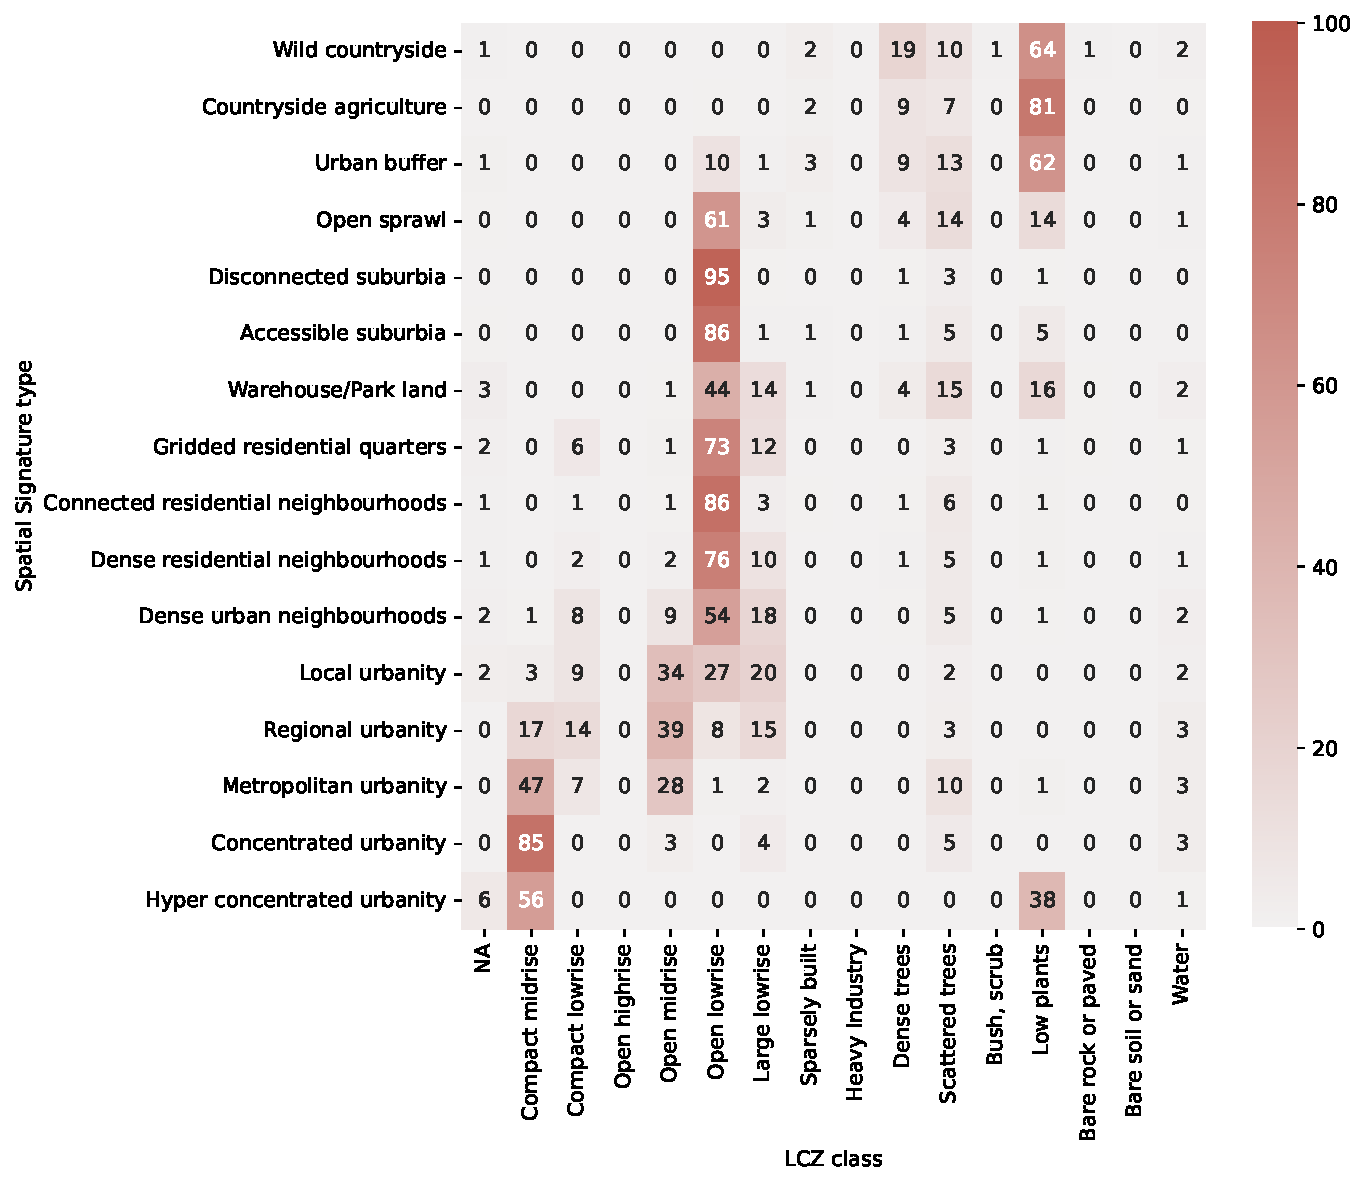
\includegraphics[width=.8\linewidth]{fig/crosstab_lcz.pdf}
    \caption{Contingency table showing frequencies (in \%) of Local Climate Zones within signature types.}
    \label{fig:crosstab_lcz}
\end{figure}

\subsection*{Summary}
None of the comparisons shows more than a moderate association, but since none of the
comparison datasets is aiming to capture the same conceptualization of space as spatial
signatures do, such a result is expected. The moderate association with both WorldPop
settlements patterns and MODUM is reassuring as both are conceptually closer to
signatures than the Urban Atlas (especially in their unsupervised design). Urban Atlas,
though very different in its aims and methods, still shows a measurable association,
which we interpret as sign that the key structural aspects forming cities are captured by both. The
comparison exercise suggests that general patterns forming cities are shared among
signatures and existing typologies. Signature types tend to form groups when we look at
their relation to comparison classes and it is not uncommon that a single signature type
is present in multiple groups linked to different classes. However, all these groups
tend to be formed based on the similarity and illustrate the granularity of the
presented classification compared to existing datasets, allowing us to distinguish, for
example, five types of signature types forming town an city centres.

